\documentclass[main.tex]{subfiles}
\begin{document}
\begin{enumerate}
% -----------------------------------------------------
% Ex 1 
% -----------------------------------------------------
\item{A spherical wave and a plane wave (same wavelength) are co-propagating on axis in air as shown in Figure \ref{fig:51}.}


\begin{enumerate}
\item{Describe the interference pattern observed at $z=100\lambda$ from the origin of the spherical wave.}

\begin{figure}
\centering\fbox{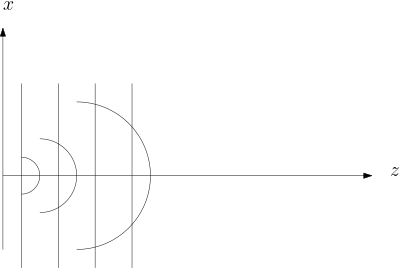
\includegraphics[height=2.0in]{figures/hw5/hw5_1.png}}
\caption{Propagating Spherical Wave and Planar Wave}
\label{fig:51}
\end{figure}

Assuming  no phase delay between the 2 waves, a plane waves $ou^{\prime}$ (what) axis propagating in $z$ can be written as 
$$g_{\mathrm{pw}}(x,z)=E_0 \exp \left \{ i \frac{2 \pi}{\lambda} z \right \}$$
where a spherical wave can be written as
$$g_{\mathrm{sw}}(x,z)= \frac{E_0}{i \lambda z} \exp \left \{ i \pi \frac{x^2}{\lambda z}  \right \} \exp \left \{ i \frac{2 \pi}{\lambda} z \right \}.$$
The interference pattern is given by the difference in phase of the 2 waves as a function of $x$ and $z$. Phase of the plane wave depends only on $z$
$$\phi_{\mathrm{pw}}(z)=\frac{2\pi}{\lambda}z$$
while the phase of the the spherical wave on both $x,z$.\\

In this regards, we will have in phase components when
$$\frac{\pi}{\lambda z}x^2 + \frac{3}{2}\pi = 2\pi m$$
which means when 
$$\Delta \phi = \phi_{pw} - \phi_{sw}$$
is an entire multiple of $2\pi$. We can solve for $x$ in Equation \ref{eq:51a1} and shown in Figure \ref{fig:51a02}.

\begin{equation}\label{eq:51a1}
\begin{array}{l}
\frac{\pi}{\lambda z}x^2 + \frac{3}{2}\pi = 2m \pi \\
x^2 = \left( 2m - \frac{3}{2} \right) \lambda z\\
m=1 \text{ \& } z=100\lambda \Rightarrow x = \pm \sqrt{\frac{1}{2}\lambda z} = \sqrt{\frac{1}{2}}10 \lambda\\
m=2 \text{ \& } z=100\lambda \Rightarrow x = \pm \sqrt{\frac{5}{2}\lambda z} = \sqrt{\frac{5}{2}}10 \lambda\\
\end{array}
\end{equation}

\begin{figure}
\centering\fbox{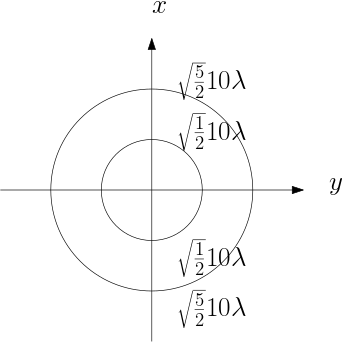
\includegraphics[height=2.0in]{figures/hw5/hw51a02.png}}
\caption{If we console the $y$ coordinate}
\label{fig:51a02}
\end{figure}

We can then solve 
$$\pi (x^2 + y^2) = (2m\pi - \frac{3}{2}\pi)\lambda z$$
which represents concentric rings of radii
$$radii = \sqrt{(2m - \frac{3}{2}) \lambda z}$$

The energy of a plane wave wave $E_{\mathrm{pl}}$ and the energy of a spherical wave $E_{\mathrm{sp}}$ are defined in Equation \ref{eq:51} where $\alpha = $.

\begin{equation}\label{eq:51}
\begin{array}{l}
{E_{\mathrm{pl}}=\left|E_{\mathrm{pl}}\right| e^{i \frac{2 \pi}{\lambda} z}} \\
{E_{\mathrm{sp}}=\frac{\left|E_{\mathrm{sp}}\right|}{\alpha z} e^{i \frac{2 \pi}{\lambda} z} e^{i \pi \frac{\left(x^{2}+y^{2}\right)}{\lambda z}}}
\end{array}
\end{equation}


At $z=100\lambda$, assuming the amplitudes $A$ of the two waves are equal we can define the phase difference between the waves in Equation \ref{eq:52}. 

\begin{equation}\label{eq:52}
\begin{array}{l}
{E_{\mathrm{pl}}=e^{i \phi_{\mathrm{pl}}} \text { where } \phi_{\mathrm{pl}}=\frac{2 \pi}{\lambda} z} \\ 
{E_{\mathrm{sp}}=e^{i \phi_{\mathrm{sp}}} \text { where } \phi_{\mathrm{sp}}=\frac{2 \pi}{\lambda} z+\frac{\pi}{\lambda z}\left(x^{2}+y^{2}\right)} \\ 
{\Delta \phi=\phi_{\mathrm{sp}}-\phi_{\mathrm{pl}}=\frac{\pi}{\lambda z}\left(x^{2}+y^{2}\right)}\end{array}
\end{equation}

The bright interference fringes occur where $\Delta \phi=2 \pi m, m=0,1,2 \ldots$ when the two waves are in phase and $\therefore  \frac{x^{2}+y^{2}}{2 z}=m \lambda$  At $z=100 \lambda \rightarrow x^{2}+y^{2}=200 \lambda^{2} m, m=0,1,2,3 \ldots $, using the circle equation $(x-x_{O})^{2}+(y-y_{O})^{2}=r^2$ from the origin we can solve for the interference pattern which is a set of concentric rings of radii $R=\lambda \sqrt{200 m}, m=0,1,2,3 \ldots$

\begin{figure}
\centering\fbox{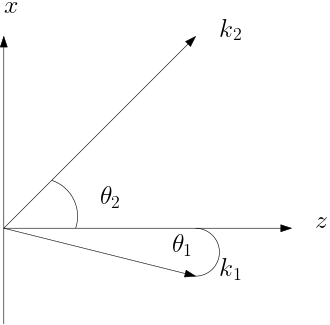
\includegraphics[height=2.0in]{figures/hw5/hw5_1b.png}}
\caption{Off-axis co-propagating plan waves}
\label{fig:52}
\end{figure}

\item{Describe the interference pattern for an off-axis co-propagating plane wave ($\theta_1 = -30$ degrees and $\theta_2 = +45$ degrees in the xz plane with respect to z) as shown in Figure \ref{fig:52}.}

The energy of a plane waves $E_{\mathrm{pl1}}$ and $E_{\mathrm{pl1}}$ are defined in Equation \ref{eq:53}.

\begin{equation}\label{eq:53}
\begin{array}{l}
{E_{\mathrm{pl1}}=\left|E_{\mathrm{pl1}}\right| e^{i \frac{2 \pi}{\lambda}(x \sin \theta_1+z \cos \theta_1)}}\\
{E_{\mathrm{pl2}}=\left|E_{\mathrm{pl2}}\right| e^{i \frac{2 \pi}{\lambda}(x \sin \theta_2+z \cos \theta_2)}}
\end{array}
\end{equation}

Assuming the amplitudes $A$ are equal at $z=100\lambda$, and intensity $I=2\left|E_{\mathrm{pl}}\right|^{2}(1+\cos \Delta \phi)$, we calculate phase delta $\Delta \phi=\phi_{\mathrm{pl2}}-\phi_{\mathrm{pl1}}$ in Equation \ref{eq:54}.

\begin{equation}\label{eq:54}
\Delta \phi= \frac{2 \pi}{\lambda} \left((x \sin \theta_2+z \cos \theta_2) - (x \sin \theta_1+z \cos \theta_1) \right)
\end{equation}

Bright fringes occur when $\Delta \phi = 2\pi m$, $m=1,2,3,\cdot$ which allows us to calculate the interference pattern in Equation \ref{eq:55}.

\begin{equation}\label{eq:55}
\lambda m =  x(\sin(45)-\sin(-30)) + z(\cos(45)-\cos(-30))
\end{equation}

\item{Is it possible to generate this kind of wave with a Michelson Interferometer?(Shown in Figure \ref{fig:53}) Please motivate and describe your answer extensively.}

\begin{figure}
\centering\fbox{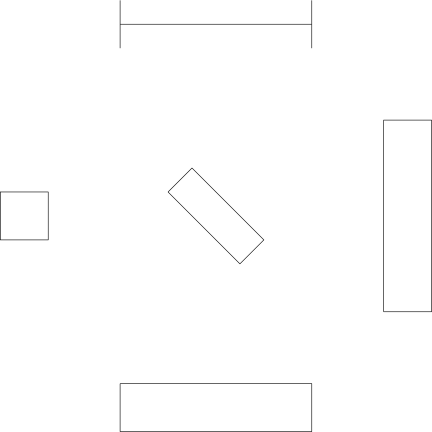
\includegraphics[height=2.0in]{figures/hw5/hw5_1c.png}}
\caption{Michelson interferometer}
\label{fig:53}
\end{figure}

%\begin{array}{l}{\text { After reflecting off the mirror, the lens is effectively imaging a point source at a }} \\ {\text { distance }(d-f)+d=2 d-f ; \text { thus it forms a point source image at } S_{i} \text { , where }} \\ {\qquad \frac{1}{S_{i}}=\frac{1}{f}-\frac{1}{S_{0}}=\frac{1}{f}-\frac{1}{2 d-f}=\frac{2(d-f)}{f(2 d-f)}} \\ {S_{i}=\frac{f(2 d-f)}{2(d-f)}} \\ {\text { If } d=f, \text { i.e. } S_{i}=\infty, \text { we get a plane back and the output is a uniform }} \\ {\text { intensity, because we would be observing the interference of two on-axis plane }} \\ {\text { waves. }} \\ {\text { If } d \neq f, \text { we get circular fringes due to the interference of a plane wave and a }} \\ {\text { spherical wave. }}\end{array}

\end{enumerate}
% -----------------------------------------------------
% Ex 2 
% -----------------------------------------------------
\item{Consider a sinusoidal amplitude grating.}
$$g_t(x)=\frac{1}{2}\left[ 1+m\cos(\frac{2\pi x}{\Lambda}) + \phi) \right]$$
at $z=0$. Illuminated by an off-axis plane wave.
$$g_{-}(x,z=0)=\exp(\frac{2\pi}{\Lambda}i \theta x)$$
\begin{enumerate}
\item{Derive the expression of $g_{\text{+}}(x,z=0)$}

For the amplitude grating, the geometry along the x-axis is considered because $z=0$. The Fresnel diffraction pattern, the field just behind the grating illuminated by the plane wave, shown in Figure \ref{fig:521} is defined in  Equation \ref{eq:521}.

\begin{figure}
\centering\fbox{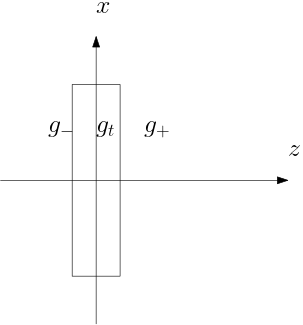
\includegraphics[height=2.0in]{figures/hw5/hw5q2a.png}}
\caption{Sinusoidal amplitude grating}
\label{fig:521}
\end{figure}

\begin{equation}\label{eq:521}
\begin{split}
g_{+}(x, z=0) & = g_{t}(x) g_{-}(x, z=0) \\
 & = \frac{1}{2}\left[ 1+m\cos(\frac{2\pi x}{\Lambda}) + \phi) \right] \exp(\frac{2\pi}{\Lambda}i \theta x)
\end{split}

\end{equation}

\item{What would be the interference pattern at infinity (Today's lecture)}
\end{enumerate}
% -----------------------------------------------------
% Ex 3 
% -----------------------------------------------------
\item{Derive the interference pattern of a plane wave passing through a double split for $D=10\lambda$. Use Huygens' principle and derive the superposition of the waves at a distance $z=L$.}\\
This problem utilizes Young's Double Slit Experiment assuming the slits are point sources. Huygenes 

\begin{figure}
\centering\fbox{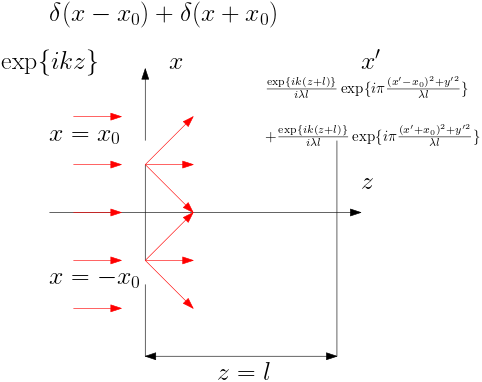
\includegraphics[width=4.0in]{figures/hw5/hw5q3.png}}
\caption{Two holes in an opaque screen with incoming plane wave on-axis}
\label{fig:53}
\end{figure}

\end{enumerate}
\end{document}